\section{Numerical result}
\label{sec:numerical-res}
In this section, we evaluate the performance in terms of average transmit power for uncoordinated CDMA and coordinated FDMA. To facilitate the discussion in the following, we call uncoordinated CDMA and coordinated FDMA simply as CDMA and FDMA. For all numerical results, we consider $P_{max} = 1$ W, $r_0 = 1000$ m,  $r_i = 50$ m, $\gamma=3$, $\mu=3$, $W = 1$ MHz, $\tau_s = 1$ sec. 
%\begin{figure}[!t]
%	\centering
%	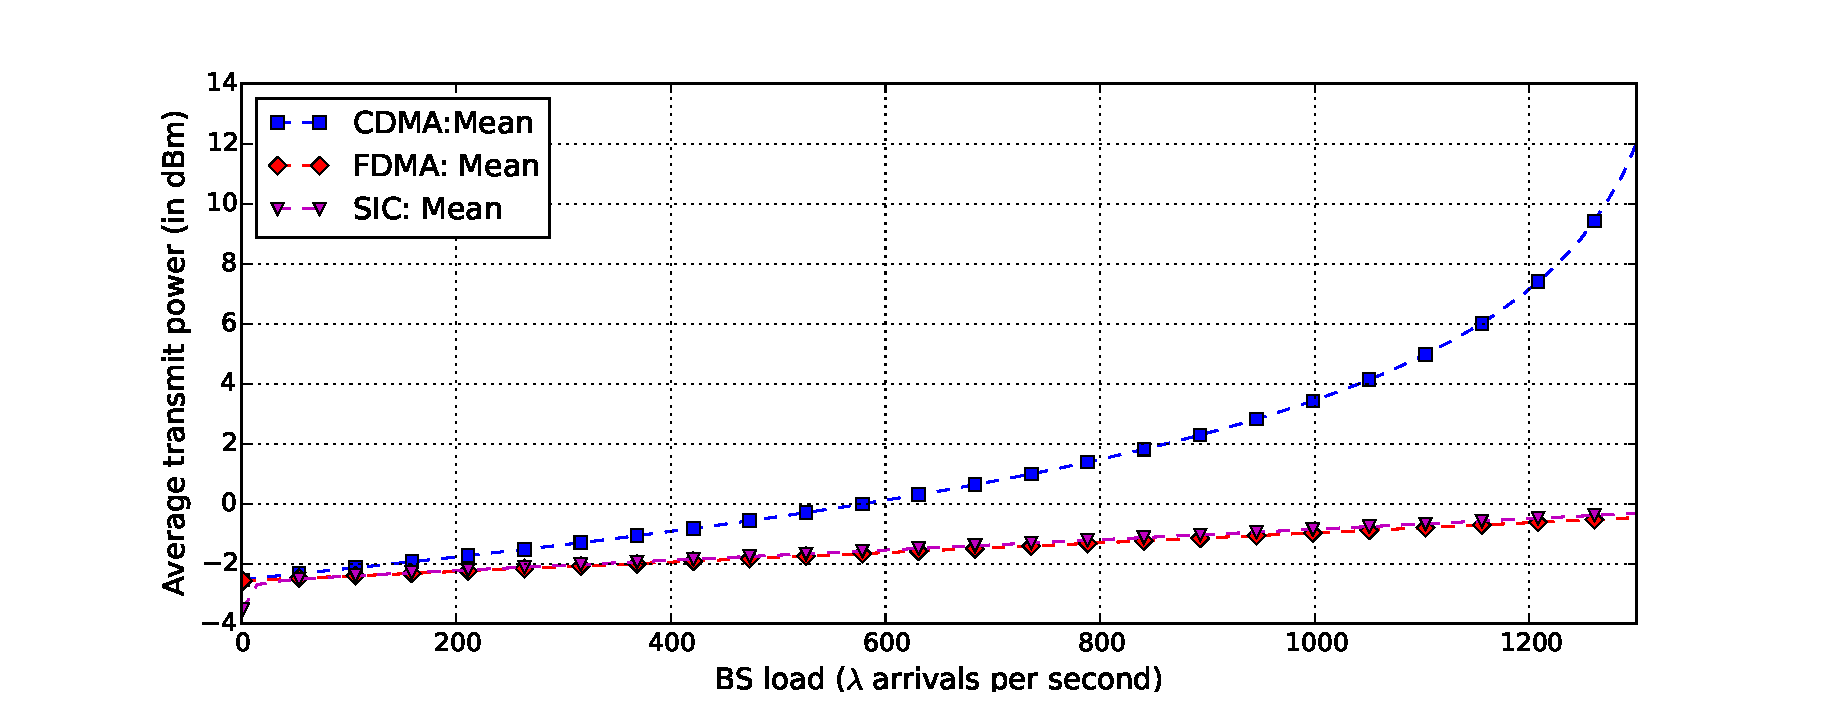
\includegraphics[width=0.5\textwidth, height=5cm]{Figures/Reproduction_Dhillon}
%	\caption{Comparison of power optimal solutions of SIC and FDMA with random access CDMA}
%	\label{fig:comparison-average-transmit-power}
%\end{figure}
\subsection{Impact of various packet length}
As discussed in previous section, the maximum supported base station load intensity is reduced when the maximum packet length increases.
The evolution of maximal packet length as to base station load intensity is illustrated in Fig.~\ref{fig:maximal-packet-length} according to inequality (\ref{ieq:packet-length-interval}). 
We evaluate the average transmit power between FDMA and CDMA under two different configurations where:\begin{inparaenum}[(i)]
	\item the packet length is constant and set as $1000$ bits;
	\item the packet length is variable varying from $1000$ bits to $3000$ bits.
\end{inparaenum}
As shown in Fig.~\ref{fig:maximal-packet-length}, to support a packet length up to $3000$ bits, the maximum base station supported load intensity is reduced to $400$ requests per second. This is the reason why the range of base station load is from $0$ to $400$ in the following figures. The evolution of power efficiency about base station load result is illustrated in Fig.~\ref{fig:Average-Transmit-Power-Variant-Target-SNR}. The curves with label reference case (CDMA or FDMA) respectively refer to the case where packet length payload $l$ is constant (namely $1000$ bits). Among all possible cases, both multiple access strategies achieve the best power efficient performance in reference case. The curve labeled \textit{\emph{CDMA:limit case}} illustrates the case where all MTC devices transfer packets with the length $3L$, which determines the upper bound limit for power consummation. All other possible cases should be between the CDMA limit case and reference case. For example, we assume packet length $l$ as a discrete random variable with distribution: $\mathbb{P}\{l=0.8L\} =0.2, \mathbb{P}\{l=1.0L\} =0.15, \mathbb{P}\{l=1.2L\} =0.15, \mathbb{P}\{l=1.6L\} =0.1, \mathbb{P}\{l=2L\} =0.1, \mathbb{P}\{l=2.5L\} =0.15, \mathbb{P}\{l=3L\} =0.15$, where $L=1000$ bits. The result associated to this configuration is shown by curve with label \textit{\emph{CDMA: general case}}.
From Fig.~\ref{fig:Average-Transmit-Power-Variant-Target-SNR}, we conclude that the coordinated FDMA strategy is more resistant to the variation of the packet length: its average transmit power increases slowly compared to that of CDMA. 

\begin{figure}[hb]
	\centering
	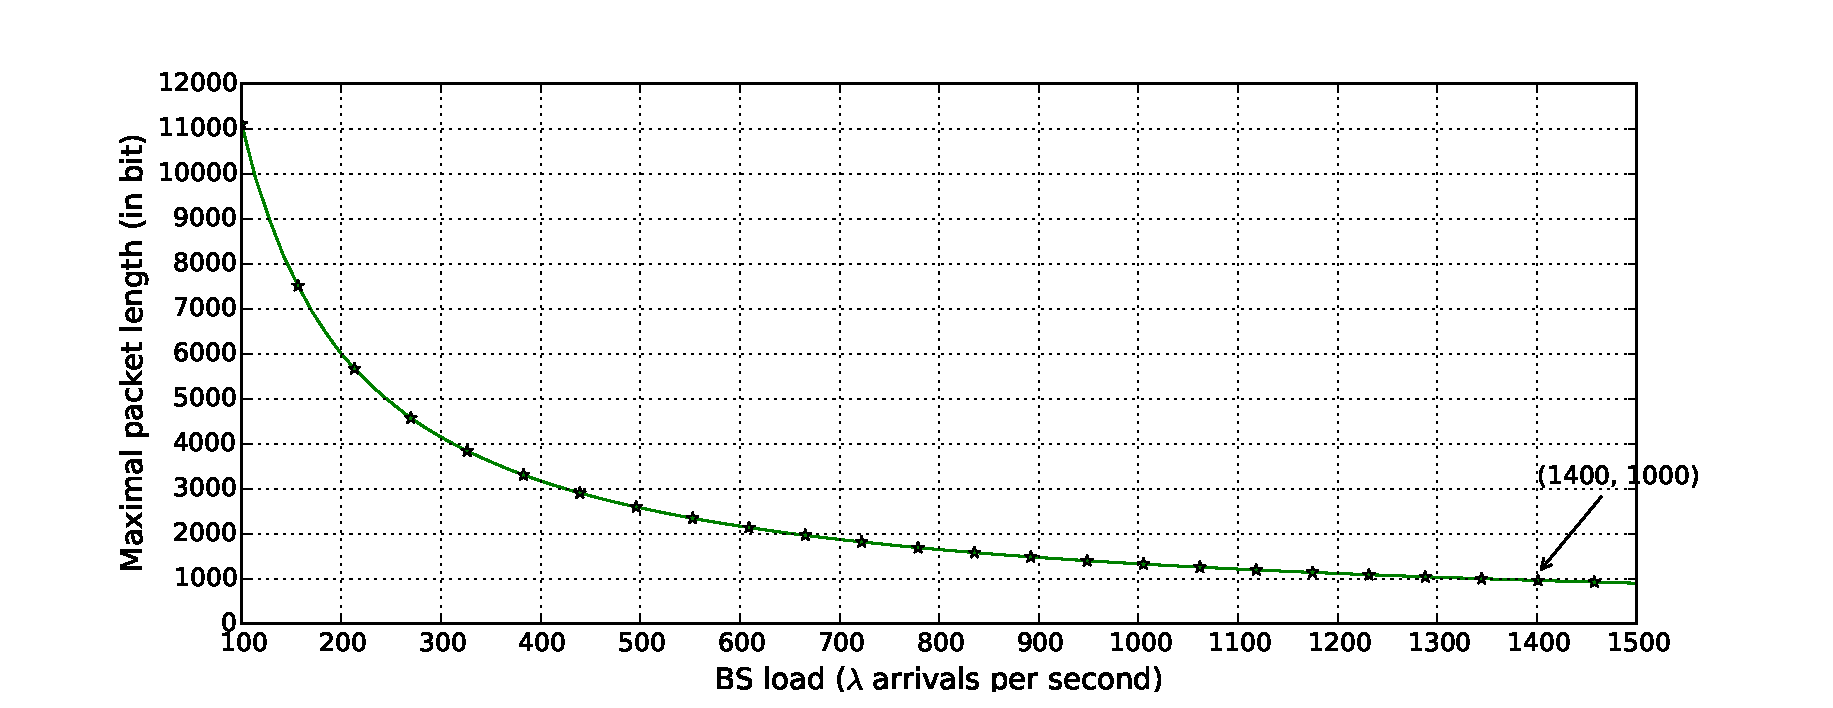
\includegraphics[width=0.5\textwidth, height=5cm]{Chapter3/Figures/Maximal-packet-length-evolution}
	\caption{Evolution of maximal packet length (in bit) with base station load intensity. For maximal packet length of 1000 bits, the maximum supported BS load is 1400.}
	\label{fig:maximal-packet-length}
\end{figure}
\begin{figure}[!tb]
	\centering
	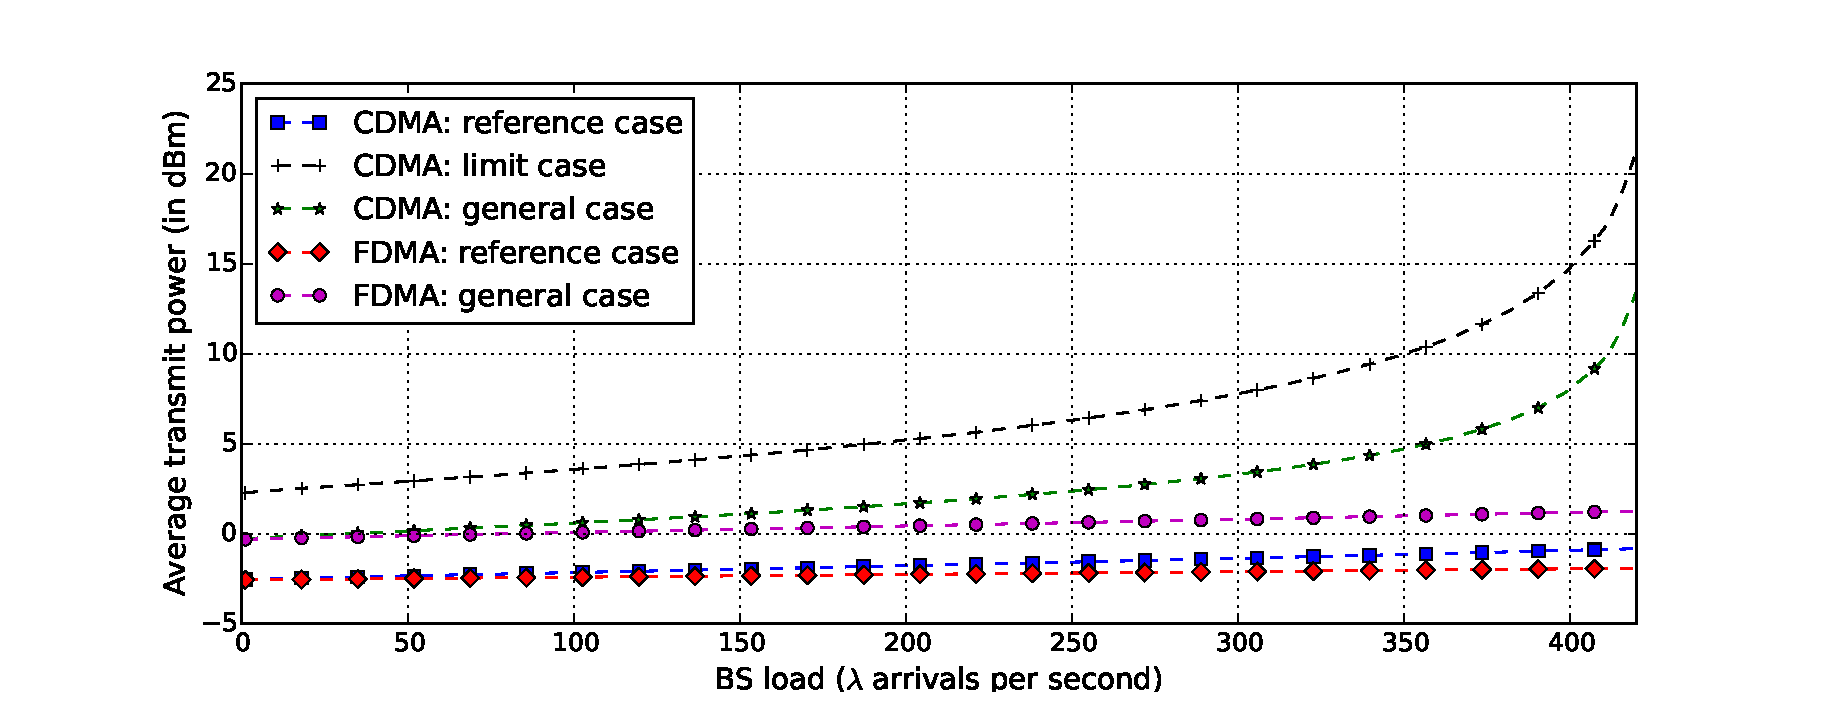
\includegraphics[width=0.5\textwidth, height=5cm]{Chapter3/Figures/Average-Transmit-Power-Variant-Target-SNR}
	\caption{Comparison of average transmit power with various packet length }
	\label{fig:Average-Transmit-Power-Variant-Target-SNR}
\end{figure}
\subsection{Imperfection of power control}
When evaluating the average transmit power under imperfect power control, we assume that the packet length $l$ is constant and set as $1000$ bits. Since it is complicated to obtain the closed-form expression for the term $C$ in formula (\ref{eq:imperfect-CDMA-transmit-power}), we take a statistical method to estimate the average transmit power for each given base station load intensity $\lambda$ and then draw the evolution curve of the average transmit power as a function of the base station load intensity. 
The numerical result where the variance of power control error $\sigma = 1$ is shown in Fig.~\ref{fig:imperfect-power-control-delta1}. The result of power control error variance $\sigma=1, 1.5$ is illustrated in Fig.~\ref{fig:imperfect-power-control-delta2}. 
The blue lines with full squares in both figures represent the case without power control error and thus serves as a reference case. The red scatter points represent the average transmit power with power control error variance $\sigma=1$, while the green scatter points are the case with power control error variance $\sigma=1.5$. From Fig.~\ref{fig:imperfect-power-control-delta1} and \ref{fig:imperfect-power-control-delta2}, the following conclusions are inferred \begin{inparaenum}[i)]
	\item the average transmit power increases when power control is imperfect;
	\item the power efficiency performance has the trend to degrade fast with a high power control error variance $\sigma$ when base station load increases.
\end{inparaenum}
\begin{figure}[!tb]
	\centering
	\includegraphics[width=0.5\textwidth, height=5cm]{Chapter3/Figures/Imperfect-power-control-CDMA-delta1-2015-1011}
	\caption{Comparison of average transmit power with power control error of variance $1$ }
	\label{fig:imperfect-power-control-delta1}
\end{figure}
\begin{figure}[!tb]
	\centering
	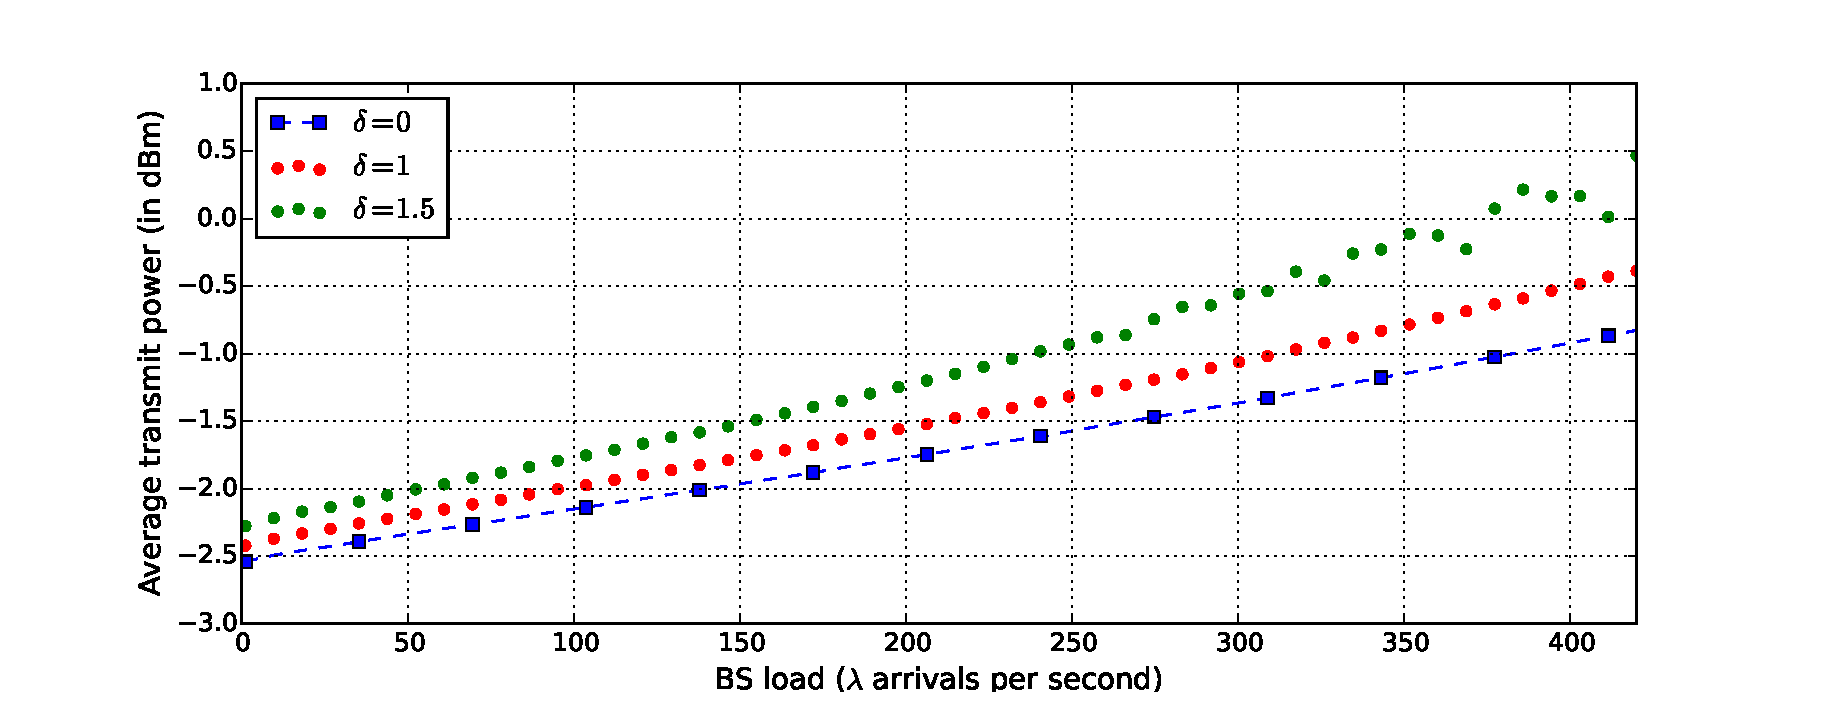
\includegraphics[width=0.5\textwidth,height=5cm]{Chapter3/Figures/Imperfect-power-control-CDMA-delta2-2015-1003}
	\caption{Comparison of average transmit power with power control error of variance $1$ and $1.5$ }
	\label{fig:imperfect-power-control-delta2}
\end{figure}